\begin{question}
\noindent Triangle $T$ is shown on the grid below.

\begin{center}
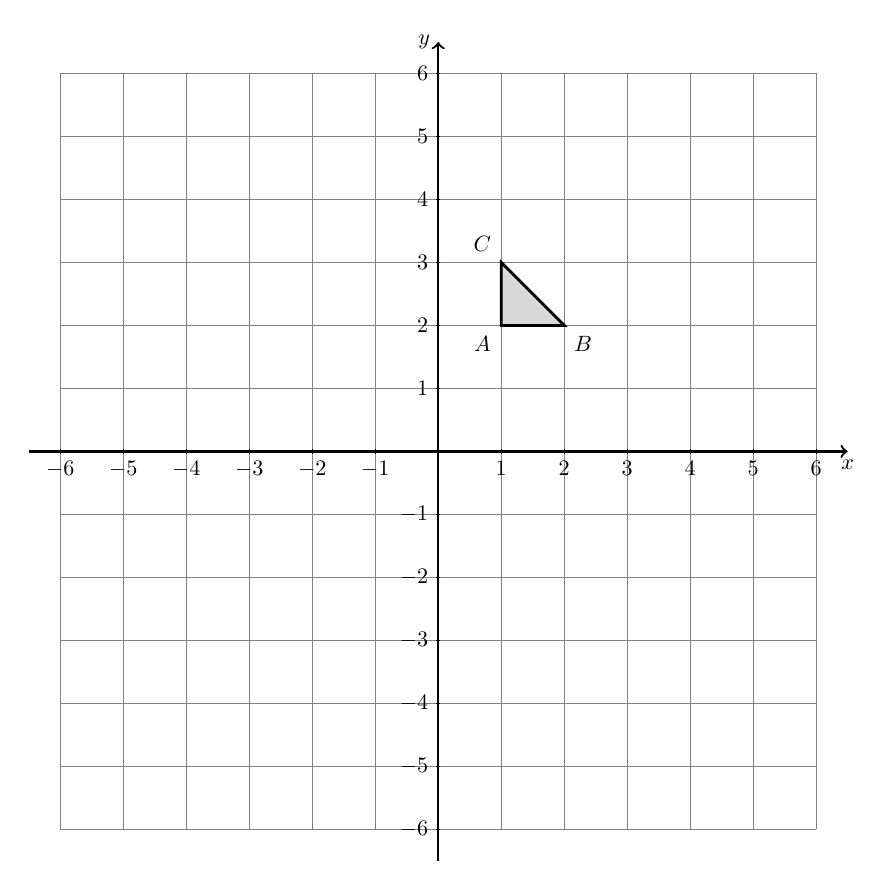
\begin{tikzpicture}[scale=0.8, transform shape]
    \def\axisLimit{6}

    \definecolor{borderColour}{HTML}{000000}
    \definecolor{fillColour}{HTML}{D8D8D8}

    % Draw grid
    \draw[step=1cm,gray,very thin] (-\axisLimit,-\axisLimit) grid (\axisLimit,\axisLimit);

    % Draw axes
    \draw[thick,->] (-\axisLimit-0.5,0) -- (\axisLimit+0.5,0) node[anchor=north] {$x$};
    \draw[thick,->] (0,-\axisLimit-0.5) -- (0,\axisLimit+0.5) node[anchor=east] {$y$};

    % Label x-axis and y-axis
    \foreach \x in {-\axisLimit,...,-1,1,2,...,\axisLimit}
        \draw (\x cm,1pt) -- (\x cm,-1pt) node[anchor=north] {$\x$};
    \foreach \y in {-\axisLimit,...,-1,1,2,...,\axisLimit}
        \draw (1pt,\y cm) -- (-1pt,\y cm) node[anchor=east] {$\y$};


    % Original triangle vertices
    \coordinate (A) at (1,2);
    \coordinate (B) at (2,2);
    \coordinate (C) at (1,3);

    \draw[fill=fillColour, draw=borderColour, line width=1pt] (A) -- (B) -- (C) -- cycle;
    \node at (0.7,1.7) {$A$};
    \node at (2.3,1.7) {$B$};
    \node at (0.7,3.3) {$C$};

\end{tikzpicture}
\end{center}

\noindent Enlarge triangle $T$ by scale factor 2, centre $P(-1,4)$.

\begin{enumerate}
    \item[(a)] Work out the coordinates of the image of each vertex of triangle $T$.

    \vspace{4cm}
    \answerplain{3}

    \item[(b)] On the grid above, draw the enlarged triangle.

    \vspace{1cm}
    \answermarks{1}
\end{enumerate}
\end{question}
